\documentclass[11pt]{article}
\usepackage{icmlko}
\begin{document}

\title{대표 수치를 더 잘 재려고 했다 --- 넷 다 실패했고, 주최자 주장이 왜 안 섞이는지는 알아냈다}
\author{월드모델 실험실}
\date{노트 357 · 2026년 8월 1일}
\maketitle

\begin{abstract}
노트 352가 대표 수치인 팝업의 95\% 구간을 $[0.257,\,0.660]$ 으로 쟀다 ---
폭 0.41 이고, 노트 351과 356의 배포 결정이 \emph{둘 다} 이 수로 갈렸다.
노트 356의 장부를 팝업에 대니 380 레코드 중 75행(80\% 버림)이고, 거르는
것은 등급이 아니라 \textbf{계수 방법}이다: \texttt{organizer\_claim} 209행이
통째로 빠진다. \texttt{lab/popupset.py} 머리말이 직접 적어 뒀다 --- ``주최자가
주장한 방문자 수를 믿을 수 있는지는 아직 아무도 안 쟀다.'' 쟀다. 팔 넷을
붙였고 \textbf{넷 다 대표를 못 올렸다.} 대신 기제를 얻었다:
\textbf{주장 라벨은 해마다 일정하게 부풀어 있다}(일평균 log10 중앙이
실측보다 2024년 $+0.27$ · 2025년 $+0.44$ · 2026년 $+0.20$ 높다). 곱셈
부풀림이라 \emph{같은 기준 안에서는} 순위가 안 다치지만 \textbf{섞으면
스피어만이 크기가 아니라 기준으로 줄을 세운다} --- 실측만 $+0.4390$ ·
주장만 $+0.1348$ · 섞으면 $+0.3088$ 이다. 노트 353 아이돌과 같은 기제가
다른 도메인에서 두 번째로 나왔다. \textbf{대표 수치의 구간은 지금 있는
레코드로는 못 좁힌다.}
\end{abstract}

\section{장부를 대표에 대 본다}

노트 356의 장부는 열 도메인을 훑는데 팝업이 빠져 있었다 --- 팝업은
\texttt{popupset} 이 따로 만들어서다. 대 봤다.

\begin{center}
\begin{tabular}{lrl}
\hline
거르는 조건 & 남는 행 & \\
\hline
전체                                & 376 & \\
$+$ 라벨 있음 $\cdot$ \texttt{scope\_usable} & 333 & \\
$+$ \texttt{counting} $\in$ (entry, participation) & \textbf{89} & $\leftarrow$ 여기서 244행이 빠진다 \\
$+$ 등급 A$\cdot$B                   & \textbf{75} & \\
\hline
\end{tabular}
\end{center}

\textbf{거르는 것은 등급이 아니다.} 등급을 A$\cdot$B 에서 A\textasciitilde{}E
로 다 풀어도 $75 \to 89$(+14)뿐이다. 빠지는 것은
\texttt{organizer\_claim} \textbf{209행}이고, 그것은 라벨 품질 문제다.

\section{팔 넷}

\begin{center}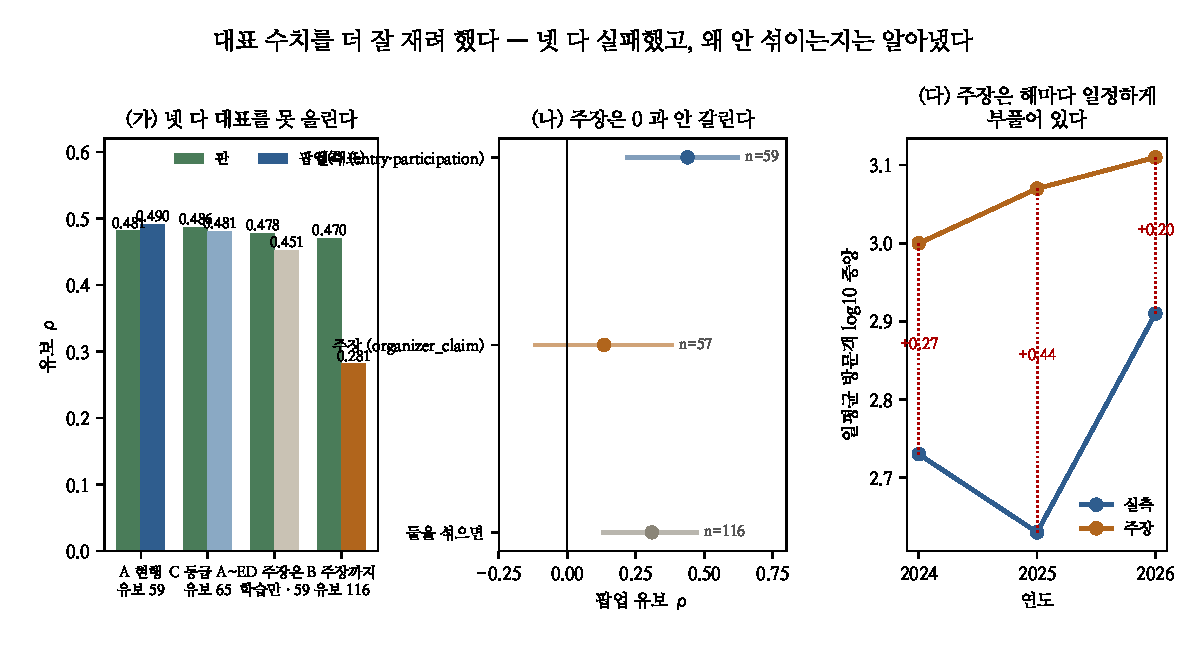
\includegraphics[width=\linewidth]{figs/claim.pdf}\end{center}

\begin{center}
\begin{tabular}{lrrrr}
\hline
팔 & 팝업 행(학습·유보) & 판 & 팝업 & 팝업 구간 폭 \\
\hline
\textbf{A 현행}          & 75 (16 · \textbf{59}) & 0.4814 & $\mathbf{0.4905}$ & 0.410 \\
C 등급 A\textasciitilde{}E & 89 (24 · 65)        & \textbf{0.4862} & 0.4810 & 0.437 \\
D 주장은 학습만          & 132 (73 · 59)         & 0.4781 & 0.4514 & --- \\
B 주장까지 유보로        & 189 (73 · \textbf{116}) & 0.4705 & 0.2813 & --- \\
\hline
\end{tabular}
\end{center}

\textbf{목적이 안 이뤄졌다.} 하려던 것은 대표 구간을 좁히는 것인데,
유보를 늘린 둘 중 C 는 $+6$ 행뿐이라 폭이 오히려 $0.410 \to 0.437$ 이고
(행이 10\% 느는 것은 폭을 5\% 줄일 뿐이라 애초에 안 보인다), B 는 유보를
두 배로 늘리는 대신 $\rho$ 를 반으로 떨어뜨린다.

\textbf{D 는 노트 127$\cdot$132 를 반복한 것인데 안 재현된다.} 그때는
분모를 59로 고정하고 학습만 $16 \to 73$ 으로 늘려 팝업이
$+0.3688 \to +0.4495$ 였다. 지금 같은 일을 하면 $0.4905 \to 0.4514$ 로
\textbf{내려간다.} 그때 팝업이 0.37 이었고 지금은 0.49 다 --- 거친 이력이
채워 주던 자리를 그 사이에 다른 것들이 채웠다.

\section{왜 안 섞이나}

미리 적어 둔 위험이 그대로 켜졌다. 계수 기준으로 갈라 재면:

\begin{center}
\begin{tabular}{lrrl}
\hline
기준 & $n$ & $\rho$ & 95\% 구간 \\
\hline
실측 (entry $\cdot$ participation) & 59 & $+0.4390$ & $[+0.211,\,+0.630]$ \\
주장 (\texttt{organizer\_claim} 등) & 57 & $+0.1348$ & $[-0.122,\,+0.388]$ \\
둘을 섞으면                        & 116 & $+0.3088$ & $[+0.126,\,+0.480]$ \\
\hline
\end{tabular}
\end{center}

차 0.304 로 미리 정한 문턱 0.15 를 넘는다 --- \textbf{안 섞는다.}
노트 353의 규약대로 연도를 맞춰서도 봤다.

\begin{center}
\begin{tabular}{lrrrr}
\hline
 & 실측 $n$ & 실측 $\rho$ & 주장 $n$ & 주장 $\rho$ \\
\hline
2025 & 40 & $+0.4508$ & 37 & $\mathbf{+0.0070}$ \\
2026 & 19 & $+0.3415$ & 20 & $+0.3456$ \\
\hline
\end{tabular}
\end{center}

\textbf{2026 은 똑같고 2025 만 무너진다.} 그리고 행이 많은 쪽이 2025 라
연도를 맞춰도 거부가 유지된다 --- 노트 353에서는 반대였다(작은 칸이
갈라서 거부가 취소됐다). \textbf{같은 검사가 한 번은 취소하고 한 번은
유지한다면 그 검사는 일하고 있는 것이다.}

\textbf{기제.} 주장 라벨의 일평균 log10 중앙이 실측보다 해마다 일정하게
높다 --- 2024년 $+0.27$ · 2025년 $+0.44$ · 2026년 $+0.20$. 1.6\textasciitilde{}2.8
배다. \textbf{곱셈 부풀림은 같은 기준 안에서는 순위를 안 건드린다} ---
그래서 주장만 재면 2026 에 $+0.3456$ 이 나온다. \textbf{다치는 것은
섞을 때다} --- 순위 하나에 두 자를 놓으면 스피어만이 ``얼마나 컸나''가
아니라 ``누가 셌나''로 줄을 세운다. 노트 353 아이돌의 연도 사이 수준
어긋남과 같은 기제이고, 이번엔 \emph{기준} 사이다.

\section{그래서 대표는 못 좁힌다}

\begin{itemize}
\item \textbf{주장 209행은 라벨이 다른 자다.} 섞을 수 없고, 학습에만 넣는
것도 지금 판에서는 손해다(D).
\item \textbf{등급을 다 풀어도 유보가 6행 는다.} 폭이 안 줄어든다.
\item \textbf{남은 길은 기준별 정규화뿐인데 그것은 과제를 바꾸는 결정이다}
--- 기준 안에서 순위를 매겨 라벨을 다시 정의하면 부풀림이 사라진다. 노트
224의 규약대로 \emph{점수로 정하면 안 되는} 종류다. 열어 둔다.
\end{itemize}

\textbf{그러니 지금 남는 사실은 이것이다: 이 실험실의 배포 결정을 두 번
가른 수(팝업)는 유보 59행에 얹혀 있고, 있는 레코드로는 그 59를 못 늘린다.}
노트 351은 팝업 $+0.0168$ 로 넣었고 노트 356은 팝업 $-0.0340$ 으로 안
뺐다 --- 둘 다 폭 0.41 짜리 수의 소수 넷째 자리로 갈린 결정이다.
\textbf{규칙이 있어서 갈렸지 수가 갈라 준 것이 아니다.}

\section{규약에 더하는 줄}

\begin{itemize}
\item \textbf{라벨을 만든 자(계수 방법 · 출처 기준)가 다르면 한 순위에
넣지 않는다.} 곱셈 부풀림은 기준 안에서는 무해하고 섞을 때만 해롭다 ---
두 번 나왔다(노트 353 연도 사이, 노트 357 기준 사이).
\item \textbf{옛 노트의 자료 결정은 지금 판에서 다시 잰다.} 노트
127$\cdot$132 의 $+0.08$ 이 지금은 $-0.04$ 다. 그때 비어 있던 자리를
그 사이에 다른 것이 채웠다.
\item \textbf{장부는 팝업에도 댄다} --- 따로 만든다고 빼 두면 제일 중요한
도메인이 감사에서 빠진다.
\end{itemize}

\section{남은 것}

\begin{center}
\begin{tabular}{ll}
\hline
갈래 & 지금 아는 것 \\
\hline
C 를 짝으로 재기 & 판 $+0.0048$ · 팝업 $-0.0095$(점추정). 짝 열둘로 \\
                & 재야 배포 규칙에 걸 수 있다. \textbf{다음 순번} \\
기준별 라벨 정규화 & 부풀림이 사라지지만 과제가 바뀐다(노트 224) \\
만화 2026 스무 건 & 노트 356. 열한 번째 채점 도메인 \\
만화가 왜 누르나 & 노트 356. 라벨 종류로는 안 갈린다 \\
\hline
\end{tabular}
\end{center}

\end{document}
